\documentclass[11pt,a4paper]{article}

% -----------------------------------------------------------------------------
% CS6868 Research Mini-Project Report Template
% -----------------------------------------------------------------------------
% Target length: 5-10 pages (including figures, excluding references).
% Compile with: latexmk -pdf main.tex
% -----------------------------------------------------------------------------

\usepackage[utf8]{inputenc}
\usepackage[T1]{fontenc}
\usepackage[margin=1in]{geometry}
\usepackage{microtype}
\usepackage{lmodern}
\usepackage{amsmath,amssymb}
\usepackage{graphicx}
\usepackage{booktabs}
\usepackage{array}
\usepackage{enumitem}
\usepackage{xcolor}
\usepackage{listings}
\usepackage{hyperref}
\usepackage{float}
\usepackage[capitalise,noabbrev]{cleveref}
\usepackage[normalem]{ulem}

\hypersetup{
  colorlinks=true,
  linkcolor=black,
  citecolor=blue!60!black,
  urlcolor=blue!60!black,
}

% --- Listings style (for code snippets) ---------------------------------------
\definecolor{codegray}{gray}{0.95}
\lstset{
  basicstyle=\ttfamily\small,
  backgroundcolor=\color{codegray},
  frame=single,
  framesep=4pt,
  breaklines=true,
  columns=fullflexible,
  keepspaces=true,
  showstringspaces=false,
}

% --- Title block --------------------------------------------------------------
\title{%
  \textbf{CS6868 Research Mini-Project} \\[0.3em]
  \Large Lock-Free Skip List%
}
\author{%
  Disha Taneja \\ \texttt{cs23b015@smail.iitm.ac.in}
  \and
  Hanumanthu Nithin \\ \texttt{cs23b025@smail.iitm.ac.in}
  \and
  Ved Prakash Dhaka\\ \texttt{cs23b086@smail.iitm.ac.in}
}
\date{\today}

\begin{document}
\maketitle

\begin{abstract}
% Briefly (150--200 words) describe the problem you tackled, your approach, the
% headline evaluation results, and the main conclusion. Readers (the graders)
% should understand the essence of your project from the abstract alone.
% \begin{abstract}
This project implements and evaluates two concurrent sorted-set data structures
in OCaml~5: a lock-free skip list following the algorithm of Herlihy et
al.~\cite{herlihy2021art} and a fine-grained locking skip list and a coarse-grained hash table implementation skip list.
All three implementations support \texttt{add}, \texttt{remove}, and \texttt{contains} on integer
keys with expected $O(\log n)$ complexity. The lock-free variant uses
compare-and-set on marked pointers to perform logical deletion, with physical
unlinking deferred to subsequent traversals. The fine-grained variant assigns
each node its own mutex and acquires predecessor locks in a globally consistent
key order to prevent deadlock. A coarse-grained hash table protected by a
single global mutex serves as a simple correctness and performance baseline.
Correctness of both lock-free and fine-grained implementations was verified using QCheck-STM, which checks
conformance to a sequential sorted-set model, and QCheck-Lin, which checks
linearisability by exhaustive interleaving search. ThreadSanitizer confirmed the
absence of data races in the lock-free variant. The fine-grained implementation
required \texttt{Atomic.t} fields for shared mutable state to suppress races
detected by ThreadSanitizer under OCaml~5's relaxed memory model. Throughput
was benchmarked under read-heavy (90\% contains), balanced (34/33/33), and
write-heavy (10\% contains) workloads across 1--16 threads on a 16-core
machine. The coarse-grained hash table outperforms both skip-list variants at
low thread counts due to its simplicity and low per-operation overhead, but
degrades sharply as thread count grows because all operations serialize on a
single lock. The fine-grained skip list consistently achieves higher throughput
than the lock-free variant across all workloads, with the gap widening under
read-heavy workloads where its lock-free \texttt{contains} path scales
particularly well. Both skip-list variants scale roughly linearly with thread
count, whereas the coarse-grained baseline does not. Traversal-length
measurements show that the lock-free variant maintains a near-constant traversal
length across all thread counts, while the fine-grained variant's traversal
length grows beyond 8--10 threads under write-heavy workloads due to increased
validation failures and lock retries under contention.
% \end{abstract}
\end{abstract}

\vspace{30em}

% =============================================================================
\section{Goals}
\label{sec:goals}
% =============================================================================

The goal of this project is to implement and evaluate a concurrent lock-free skip list in OCaml 5. The data structure supports the standard sorted-set operations \texttt{add}, \texttt{remove}, and \texttt{contains} on integer keys. The lock-free implementation uses atomic compare-and-set operations together with marked pointers, following the Harris-list style technique, where deletion is divided into logical deletion and physical unlinking.

This problem is interesting because skip lists provide expected logarithmic-time search, insertion, and deletion without requiring rotations, as in balanced binary search trees. In a concurrent setting, avoiding rotations is valuable because large structural changes can create synchronization bottlenecks and complicated interleavings. A skip list instead maintains multiple linked-list levels using randomized promotion, so updates are relatively local while higher levels provide fast traversal. This makes skip lists a good case study for comparing different synchronization strategies on a non-trivial search data structure.

The project connects directly to the course topics on concurrent linked lists, compare-and-set based synchronization, lock-free algorithms, fine-grained locking, logical versus physical deletion, and linearizability. The lock-free skip list extends the Harris linked-list idea from Lecture 07 to a multi-level structure: nodes are first logically deleted by marking pointers and are then physically unlinked by later traversals. The fine-grained locking baseline connects to hand-over-hand and local locking techniques, while the testing part connects to the course emphasis on verifying concurrent objects against a sequential specification.

Another goal is to compare the lock-free implementation against a fine-grained locking skip list baseline. Both implementations provide the same abstract sorted-set interface, but they use different synchronization mechanisms. The lock-free version relies on atomic retry loops and helping during traversal, while the fine-grained version uses locks to protect local predecessor and successor regions during updates.

The project also aims to verify correctness using QCheck-Lin and QCheck-STM, run ThreadSanitizer on the lock-free variant, and benchmark throughput under read-heavy, balanced, and write-heavy workloads across multiple thread counts. In addition, traversal lengths are measured under concurrent modification to study whether contention causes excessive retries in the lock-free variant.

The research question, taken from the project statement, is: how does the lock-free skip list's throughput scale compared to a fine-grained locking skip list across different workload mixes, and does the multi-level structure amplify or mitigate the retry overhead of lock-free operations compared to a single-level Harris list?
% =============================================================================
\section{Background}
\label{sec:background}
% =============================================================================

% Summarise the algorithm or technique at a level that a classmate who has
% attended the lectures but not read the paper can follow. Cite the primary
% references. If helpful, include a small figure or
% pseudo-code listing.


A \emph{skip list}~\cite{pugh1990skip} is a probabilistic data structure that
maintains a sorted set using multiple levels of linked lists. Level~0 contains
all elements in sorted order, while higher levels contain progressively fewer
elements and act as “express lanes” for faster traversal. A search starts at
the highest level, moves right while the next key is smaller than the target,
and drops down one level when it would overshoot. This results in expected
$O(\log n)$ time for search, insertion, and deletion.


\begin{figure}[h]
\centering
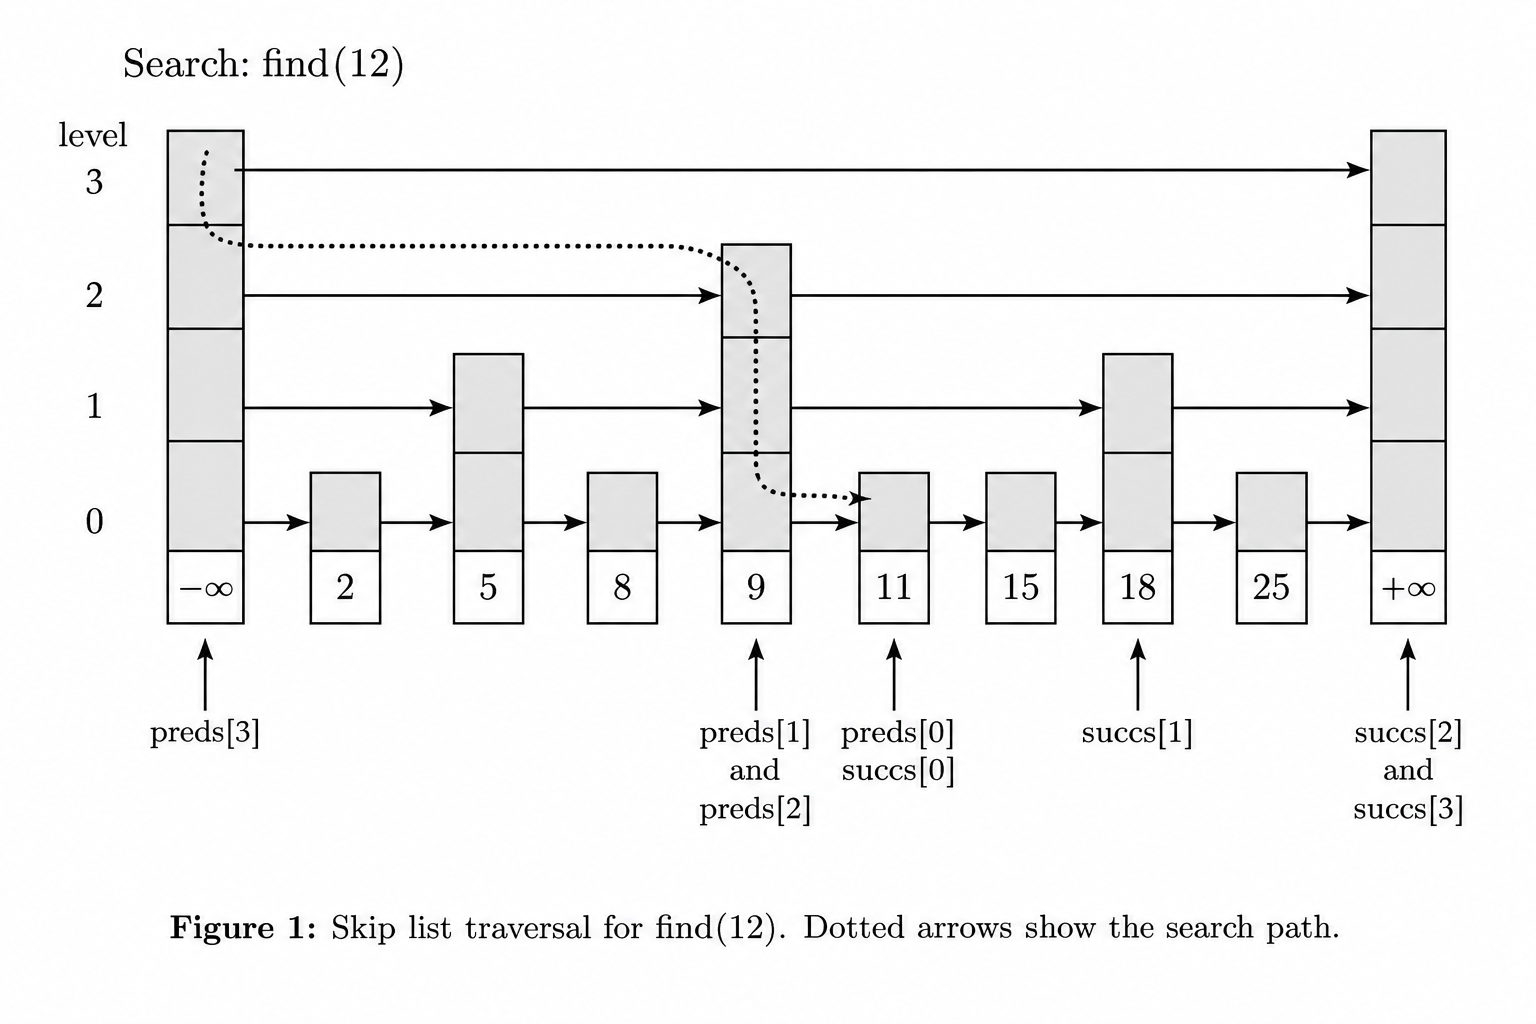
\includegraphics[width=0.95\linewidth]{./skiplist_traversal.png}
\caption{Skip list traversal for \texttt{find(12)}. The search proceeds by moving
right at each level and dropping down when necessary. The \texttt{preds} and
\texttt{succs} arrays record predecessors and successors at each level.}
\label{fig:skiplist-traversal}
\end{figure}

In a concurrent setting, operations must safely update multiple levels of the
structure. Two main approaches are used.

\emph{Fine-grained locking.}
Each node is associated with a mutex, and update operations lock a small set of
predecessor nodes before modifying pointers. After acquiring locks, the
structure is validated to ensure it has not changed due to concurrent updates.
Deletion is performed in two phases: logical marking followed by physical
unlinking. A \texttt{fully\_linked} flag ensures that partially inserted nodes
are not observed, and locks are acquired in a consistent order to prevent
deadlock.

\emph{Lock-free skip list.}
This approach avoids locks and instead uses compare-and-set (CAS) on pointers
augmented with a mark bit. Deletion is performed by marking a node’s next
pointers (logical deletion), while physical removal is carried out by other
threads during traversal (\emph{helping}). Insertion first links the node at
level~0 (the linearisation point) and then attempts to link higher levels,
retrying if concurrent updates interfere. The \texttt{contains} operation is
wait-free, as it only performs reads and skips marked nodes.

Both implementations aim to satisfy linearisability
ensuring that each operation appears to take effect atomically at some point
between its invocation and response.

% Example listing:
% \begin{lstlisting}[language=caml,caption={Sketch of the algorithm.},label={lst:algo}]
% let foo x = ...
% \end{lstlisting}

% =============================================================================

\section{Tasks Undertaken}
\label{sec:tasks}

\subsection{Implementation}

\subsubsection{Lock-free skip list}
\label{sec:lockfree-impl}

The main implementation is a lock-free skip list over integer keys. It provides the operations \texttt{add}, \texttt{remove}, and \texttt{contains}.The abstract set is defined by the bottom-level list, while higher levels act as shortcuts to speed up traversal.

Each node stores a key, a randomly chosen top level, and an array of next pointers.
\begin{lstlisting}[language=caml,caption={Node type for lock-free skip list.},label={lst:lockfree-node}]
type node = {
  key       : int;
  top_level : int;
  next      : node Atomic_markable_ref.t array;
}
\end{lstlisting}
Each next pointer is represented using an \texttt{Atomic\_markable\_ref}, which stores both a reference and a Boolean mark bit. The mark bit is used to distinguish ordinary links from links belonging to logically deleted nodes. The markable reference abstraction provides atomic read operations and a compare-and-set operation over both the reference and the mark bit. This is the OCaml equivalent of the atomic markable reference used in standard lock-free skip-list descriptions~\cite{herlihy2021art}.

The \texttt{find} procedure is the main helper used by update operations. It traverses the skip list from the highest level down to level 0, maintaining predecessor and successor arrays for the search key. While traversing, if it observes a marked node, it attempts to physically unlink that node by applying compare-and-set on the predecessor's next pointer. If this cleanup CAS fails, the search restarts because the local predecessor/successor information may have become stale. This means that traversal also performs helping: operations that encounter logically deleted nodes help remove them from the structure.

Insertion first calls \texttt{find}. If the key is already present in the bottom-level list, \texttt{add} returns false. Otherwise, a new node is created with a random height, and its next pointers are initialized using the successors returned by \texttt{find}. The implementation first attempts to splice the node into the bottom-level list using \texttt{Atomic.compare\_and\_set}. This bottom-level successful CAS is the linearization point of a successful \texttt{add}, because from that point onward the key is part of the abstract set. After this, the implementation attempts to link the same node into higher levels. If linking at a higher level fails because another thread changed that list,\texttt{find} is called again to refresh the predecessor and successor arrays before retrying that level.

Removal also starts with \texttt{find}. If the key is not found in the bottom-level list, \texttt{remove} returns false. If the key is found, the implementation marks the node's higher-level links first and then attempts to mark the bottom-level link. Marking the bottom-level link is the linearization point of a successful \texttt{remove}, since the abstract set is defined by unmarked nodes in the bottom level. After successfully marking the bottom-level link, the operation calls \texttt{find} again to help physically unlink the removed node.

The \texttt{contains} operation performs a traversal without modifying the list. It moves from higher levels to lower levels and skips over marked nodes when they are encountered.Since \texttt{contains} is expected to be the most frequent operation, it is implemented as a wait-free operation,  it does not acquire locks, does not perform compare-and-set updates, and therefore avoids blocking behind concurrent \texttt{add} or \texttt{remove} operations.~\cite{herlihy2021art}.

% ---------------------------------------------------------------------------
% Section 2.2 — Fine-Grained Locking Skip List (replaces the empty subsubsection)
% ---------------------------------------------------------------------------
\subsubsection{Fine-grained locking skip list}
\label{sec:finegrain-impl}

The fine-grained locking skip list provides the same abstract sorted-set
interface as the lock-free variant: \texttt{add}, \texttt{remove}, and
\texttt{contains} over integer keys.  It uses a different synchronisation
strategy: each node carries its own \texttt{Mutex.t}, and update operations
lock a small set of predecessor nodes rather than the entire structure.

Each node stores a key, a randomly chosen top level, a per-node mutex, a
logical-deletion flag \texttt{marked}, a visibility flag
\texttt{fully\_linked}, and an array of next pointers. 
% \sout{Because \texttt{find}
% traverses next pointers without holding any lock, all three mutable fields are
% represented as \texttt{Atomic.t} values so that lockless reads and locked
% writes do not produce data races detected by ThreadSanitizer:}

\begin{lstlisting}[language=caml,caption={Node type for fine grained skip list.}]
type node = {
  key          : int;
  top_level    : int;
  next         : node option Atomic.t array;
  lock         : Mutex.t;
  marked       : bool Atomic.t;
  fully_linked : bool Atomic.t;
}
\end{lstlisting}

\vspace{3em}
The helper \texttt{find} walks the list from the highest level down to level~0,
recording predecessor and successor arrays for the search key and returning the
highest level at which the key was found (or $-1$ if absent).  All reads go
through \texttt{Atomic.get} to avoid races with concurrent writes.

% A second helper, \texttt{find\_preds}, is used exclusively by
% \texttt{physical\_remove}.  Unlike \texttt{find}, it fills only the
% \texttt{preds} array and stops at nodes whose key is strictly less than the
% target.  This is necessary because after a node is logically deleted
% (\texttt{marked~:=~true}) it remains physically in the list, so a call to
% \texttt{find} cannot reliably identify its predecessors across all retry
% scenarios; \texttt{find\_preds} is immune to this because it navigates
% by key comparison alone.
% \vspace{1em}

The \texttt{lock\_unique\_sorted} is used in both \texttt{add} and the 
physical-removal phase of \texttt{remove} to hold
several predecessor locks simultaneously.  A naive bottom-up locking order
causes deadlock when two concurrent operations have overlapping predecessor
sets and acquire them in opposite orders.  The function \texttt{lock\_unique\_sorted} eliminates this by collecting the distinct predecessor nodes and then acquiring their mutexes in that order. Since the input \texttt{preds} array produced by \texttt{find()} is already in non-decreasing key order, every domain acquires locks in a consistent global order, making circular wait impossible.

% \begin{lstlisting}[language=caml,caption={Sorted lock acquisition.}]
% let lock_unique_sorted preds top_level =
%   let seen = ref [] in
%   for level = bottom_level to top_level do
%     let pred = preds.(level) in
%     if not (List.exists (fun n -> n == pred) !seen) then
%       seen := pred :: !seen
%   done;
%   List.iter (fun n -> Mutex.lock n.lock) !seen;
%   !seen
% \end{lstlisting}

\vspace{1em}
The \texttt{add} function assigns a random height using a geometric distribution, then
enters a retry loop.  On each attempt it calls \texttt{find} to locate
predecessor and successor arrays.  If the key is already present and not
marked, \texttt{add} spins until \texttt{fully\_linked} is set or the
node becomes marked (to avoid an infinite spin when \texttt{remove} marks a
node before \texttt{add} finishes observing it).  If the key is absent,
\texttt{add} calls \texttt{lock\_unique\_sorted}, validates that no predecessor
was concurrently marked and that each predecessor still points to the recorded
successor, splices the new node in at every level, sets
\texttt{fully\_linked~:=~true} as the publishing point, then releases all
locks.  The successful bottom-level update (the write to
\texttt{preds.(0).next.(0)}) under the predecessor lock is the linearisation
point of a successful insert.

% The \texttt{add} function assigns a random height using a geometric distribution and then
% enters a retry loop. On each iteration it calls \texttt{find} to obtain the predecessor and
% successor arrays. Several situations cause the operation to retry. First, if the key is found
% but the node is not yet \texttt{fully\_linked}, the operation spins until either
% \texttt{fully\_linked} becomes true or the node becomes \texttt{marked}; this avoids returning
% an incorrect result while another concurrent insertion is still in progress. Second, if the key
% is absent, the operation proceeds to lock the required predecessors and then validates the
% snapshot: if any predecessor is marked or no longer points to the recorded successor, the
% snapshot is stale and the operation releases all locks and restarts from \texttt{find}. This
% retry is necessary because concurrent updates may have modified the structure between the
% initial traversal and lock acquisition.

% If validation succeeds, the new node is spliced into the list level by level, and
% \texttt{fully\_linked := true} is set as the publishing step. The \texttt{fully\_linked} flag is
% essential because insertion is a multi-step process: the node is first linked into the structure
% but is not yet logically part of the set until all its levels are connected. Without this flag,
% other operations (especially \texttt{contains} or concurrent \texttt{add}) could observe a
% partially inserted node and incorrectly treat it as present, violating linearizability. By
% delaying visibility until \texttt{fully\_linked} is set, the implementation ensures that a node
% becomes visible to other threads only after insertion is complete. The successful bottom-level
% update (the write to \texttt{preds.(0).next.(0)}) under the predecessor lock acts as the
% linearisation point of a successful insert.

% \paragraph{Removal (\texttt{remove}).}
\vspace{1em}
The Removal(\texttt{remove}) is split into two phases to prevent retry-state leakage between
attempts. Phase~1 — logical deletion (\texttt{find\_and\_mark}).
\texttt{find} locates the candidate node.  If it is not yet \texttt{fully\_linked}
or is already \texttt{marked}, the function returns \texttt{None} immediately.
Otherwise it acquires only the candidate's own lock, re-checks
\texttt{marked} under the lock (to handle concurrent removers), sets
\texttt{marked~:=~true}, and releases the lock.  Setting the mark is the
linearisation point of a successful remove.

Phase~2 — physical unlinking (\texttt{physical\_remove}).
\texttt{find} refreshes the predecessor array for the now-marked victim.
\texttt{lock\_unique\_sorted} acquires predecessor locks in key order.  Each
predecessor is validated: it must not itself be marked, and its next pointer at
that level must still point to the victim.  If validation fails, all locks are
released and the phase retries.  On success, each predecessor's next pointer is
swung past the victim using \texttt{Atomic.set}, and the locks are released.

% \paragraph{Membership query (\texttt{contains}).}
% \vspace{1em}
The \texttt{contains} function calls \texttt{find} without acquiring any lock.  It returns
\texttt{true} only if the found node is \texttt{fully\_linked} and not
\texttt{marked}.  The linearisation point is the read of \texttt{marked} at
the bottom level.

\vspace{1em}

In the lock-free skip list, physical removal is performed during \texttt{find} as part of traversal because there are no locks to guarantee exclusive access to a local region of the structure. Instead, the algorithm relies on \emph{helping}: when a thread encounters a logically deleted (marked) node, it attempts to unlink it using compare-and-set before proceeding. This ensures that marked nodes do not accumulate and that traversal remains efficient, while also allowing any thread to complete pending work left by others. Restricting physical removal to \texttt{remove} in the lock-free setting would be problematic, because once a node is logically marked, the removing thread may be delayed or fail before completing the unlinking; without helping, such nodes would remain indefinitely, degrading performance and potentially causing long retry chains for other operations.

In contrast, the fine-grained locking skip list performs physical removal inside \texttt{remove}, after acquiring locks on the relevant predecessors. This provides a safe and controlled context for pointer updates without interference. Placing physical removal inside \texttt{find} in the fine-grained design would require acquiring locks during traversal, turning \texttt{find} into a blocking operation. This would significantly reduce concurrency and harm performance, especially for read-heavy workloads where \texttt{find} and \texttt{contains} are expected to be fast and non-blocking. Thus, lock-free designs distribute cleanup across traversals via helping to ensure progress without locks, whereas fine-grained locking confines cleanup to update operations to preserve efficient, lock-free reads.
% \paragraph{Correctness properties.}
% Table~\ref{tab:fg-props} summarises the main invariants maintained by the
% implementation.

% \begin{table}[h]
% \centering
% \small
% \begin{tabular}{@{}ll@{}}
% \toprule
% \textbf{Property} & \textbf{Mechanism} \\
% \midrule
% No deadlock            & Predecessors locked in ascending key order \\
% No data race on next   & \texttt{node option Atomic.t array} \\
% No data race on flags  & \texttt{bool Atomic.t} for \texttt{marked} and \texttt{fully\_linked} \\
% Safe lockless reads    & \texttt{find}/\texttt{contains} use \texttt{Atomic.get} throughout \\
% Logical before physical & \texttt{find\_and\_mark} completes before \texttt{physical\_remove} starts \\
% \bottomrule
% \end{tabular}
% \caption{Key correctness invariants of the fine-grained locking skip list.}
% \label{tab:fg-props}
% \end{table}

\subsubsection{Coarse-grained hash-table baseline}
\label{sec:coarsegrain-impl}
A coarse-grained hash table using a single global mutex provides a simple baseline for comparison. Each operation (\texttt{add}, \texttt{remove}, \texttt{contains}) acquires the mutex, performs the table operation, and releases the lock. While this avoids retry loops and multi-level complexity, it suffers from high contention under concurrent access. This baseline clarifies the trade-off: global locking guarantees simplicity and safety but stalls all concurrent operations, whereas lock-free and fine-grained approaches aim to improve parallelism at the cost of added complexity.

\subsection{Testing and Verification}

\subsubsection{Manual tests}
\label{sec:manual-tests}

Manual tests for the lock free skiplist mainly checked whether the implementation behaved like a normal set for \texttt{add}, \texttt{remove}, and \texttt{contains}. The cases included insertion into an empty list, duplicate insertion, removal of an existing key, removal of an absent key, membership checks after updates, and re-addition of a key after deletion.

A few implementation-specific edge cases were also tested, such as negative keys, zero, large keys, and the case where \texttt{max\_level = 0}. The last case is useful because the skip list becomes a single-level lock-free list, so it checks whether the bottom-level logic works correctly even without higher-level shortcut links.

For concurrent testing, multiple domains were used to run operations at the same time. The tests included insertion of disjoint ranges, removal of pre-inserted keys, and mixed \texttt{add}, \texttt{remove}, and \texttt{contains} operations. Same-key races were also tested, where many domains try to add or remove the same key. In such cases, only one successful add or remove should be reported.

These tests do not prove linearizability, but they helped catch basic bugs before moving to QCheck-STM and QCheck-Lin.

\subsubsection{QCheck-STM}
\label{sec:qcheck-stm}

QCheck-STM was used to test both implementations against a sequential reference
model. The model state is an \texttt{int list} representing the set contents in
sorted order, starting empty.  
  
Keys are drawn from $[0, 20]$ so that concurrent operations frequently target
the same key, maximising the chance of exposing race conditions and incorrect
return values.

 
 

\subsubsection{QCheck-Lin}
\label{sec:qcheck-lin}
 
QCheck-Lin provides a direct linearisability test by exhaustive interleaving
within \textt{add}, \texttt{remove} and \texttt{contains}.  


\subsubsection{ThreadSanitizer}
The ThreadSanitizer run did not report data races in both fine-grained and  lock-free skip-list implementations
% =============================================================================
\section{Evaluation}
\label{sec:evaluation}
% =============================================================================

\subsection{Experimental Setup}

\textit{Hardware and configuration: 16 cores on a intel i7- 13th gen processor, with 16 GB RAM}

We have two kinds of benchmarks, one for measuring throughput and other one for measuring avg number of nodes traversed per operation. We will present each of them in detail below.

\subsection{Throughput Results}
\textit{The below implementation was inspired from benchmarking done for various kinds of lists in lecture 7}

We tested three workload mixes to exercise different contention regimes:
\begin{itemize}
  \item \textbf{Read-heavy:} 90\% contains, 5\% add, 5\% remove.
  \item \textbf{Equal:} 34\% contains, 33\% add, 33\% remove.
  \item \textbf{Write-heavy:} 10\% contains, 45\% add, 45\% remove.
\end{itemize}
\textbf{And also another Measurement, which involves variable \%contains and fixed threads (14 here)}
\newline
\vspace{1cm}

\textbf{Measurement methodology}: For throughput we preload the data structure with the configured initial size, run a short warm-up phase (1 run of what an benchmark would be like) to stabilise caches and allocator state, then performed the measured runs. Each measured run spawns \texttt{num\_threads} domains and runs for the configured \texttt{duration} (seconds); workers perform random operations according to the workload mix and increment a shared atomic counter. Throughput for a run is computed as total operations divided by elapsed time (ops/sec). We repeat the measured run \texttt{runs} times, call \texttt{Gc.compact()} between runs to reduce memory-state variance, and report median and average throughput across runs. \texttt{Runs} was fixed to 3 and \texttt{duration} = 2 secs.

\newline
\vspace{1cm}
\textbf{Conclusions}:
\newline
Figure 2-5 represent the plots. The hashtbl variant works significantly better than skiplist variants in low contention but performance declines significantly as no of threads increase, which is expected as majority of the work is under a lock. Among skiplist variants we didn't have any prior expectation of different they are going to be among each other, but finegrain version perfroms better than lockfree variant in all three different workloads. Both algorithms scaled well without any major breakdown (the right edge of the graph seems bit different probably becuase of reaching our hardware limits i.e in number of cores). Individually both have a almost linear growth, with finegrain version having more sharper growth. However, under write heavy load the both the variants were comparatively more closer in each other in performance, implying finegrain doesn't grow as sharply under heavy write loads (which is also being implied by the growth in throughput towards heavy contains in fig 5). 

\begin{figure}[H]
  \centering
  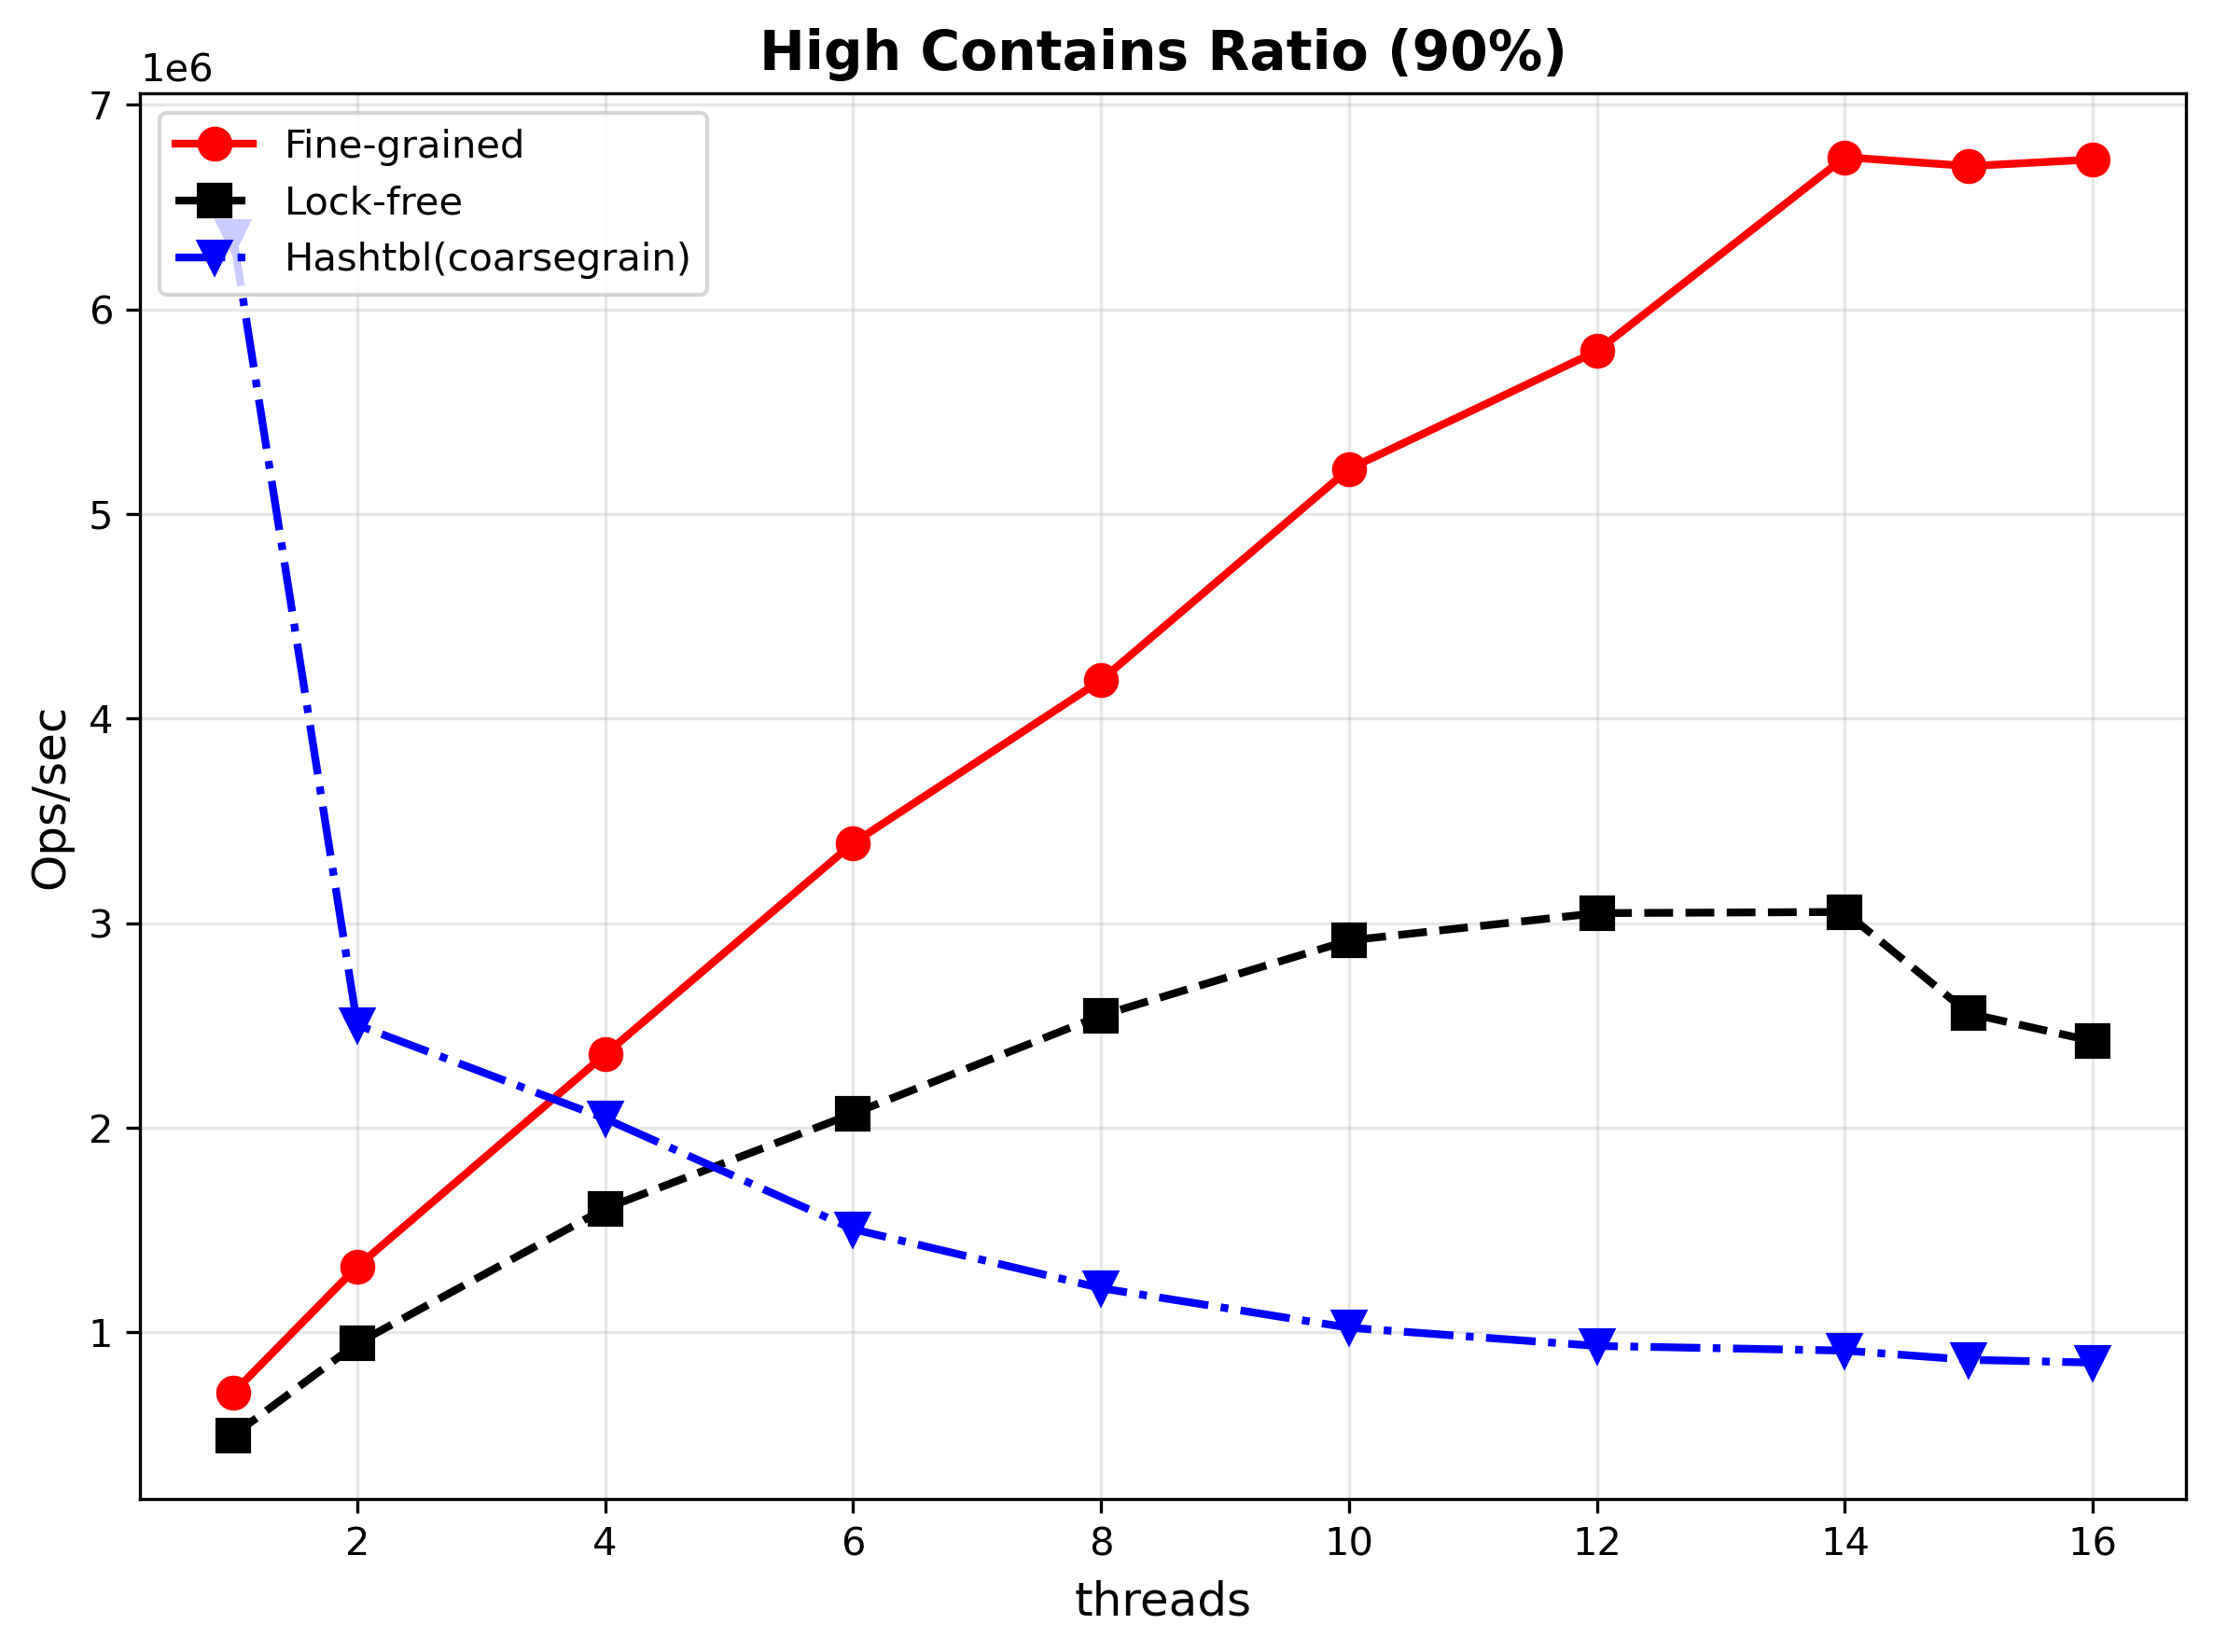
\includegraphics[width=0.85\linewidth]{./plots/plot_high_contains.png}
  \caption{Throughput comparison across implementations and thread counts under Read-heavy workload.}
\end{figure}
 
\begin{figure}[H]
  \centering
  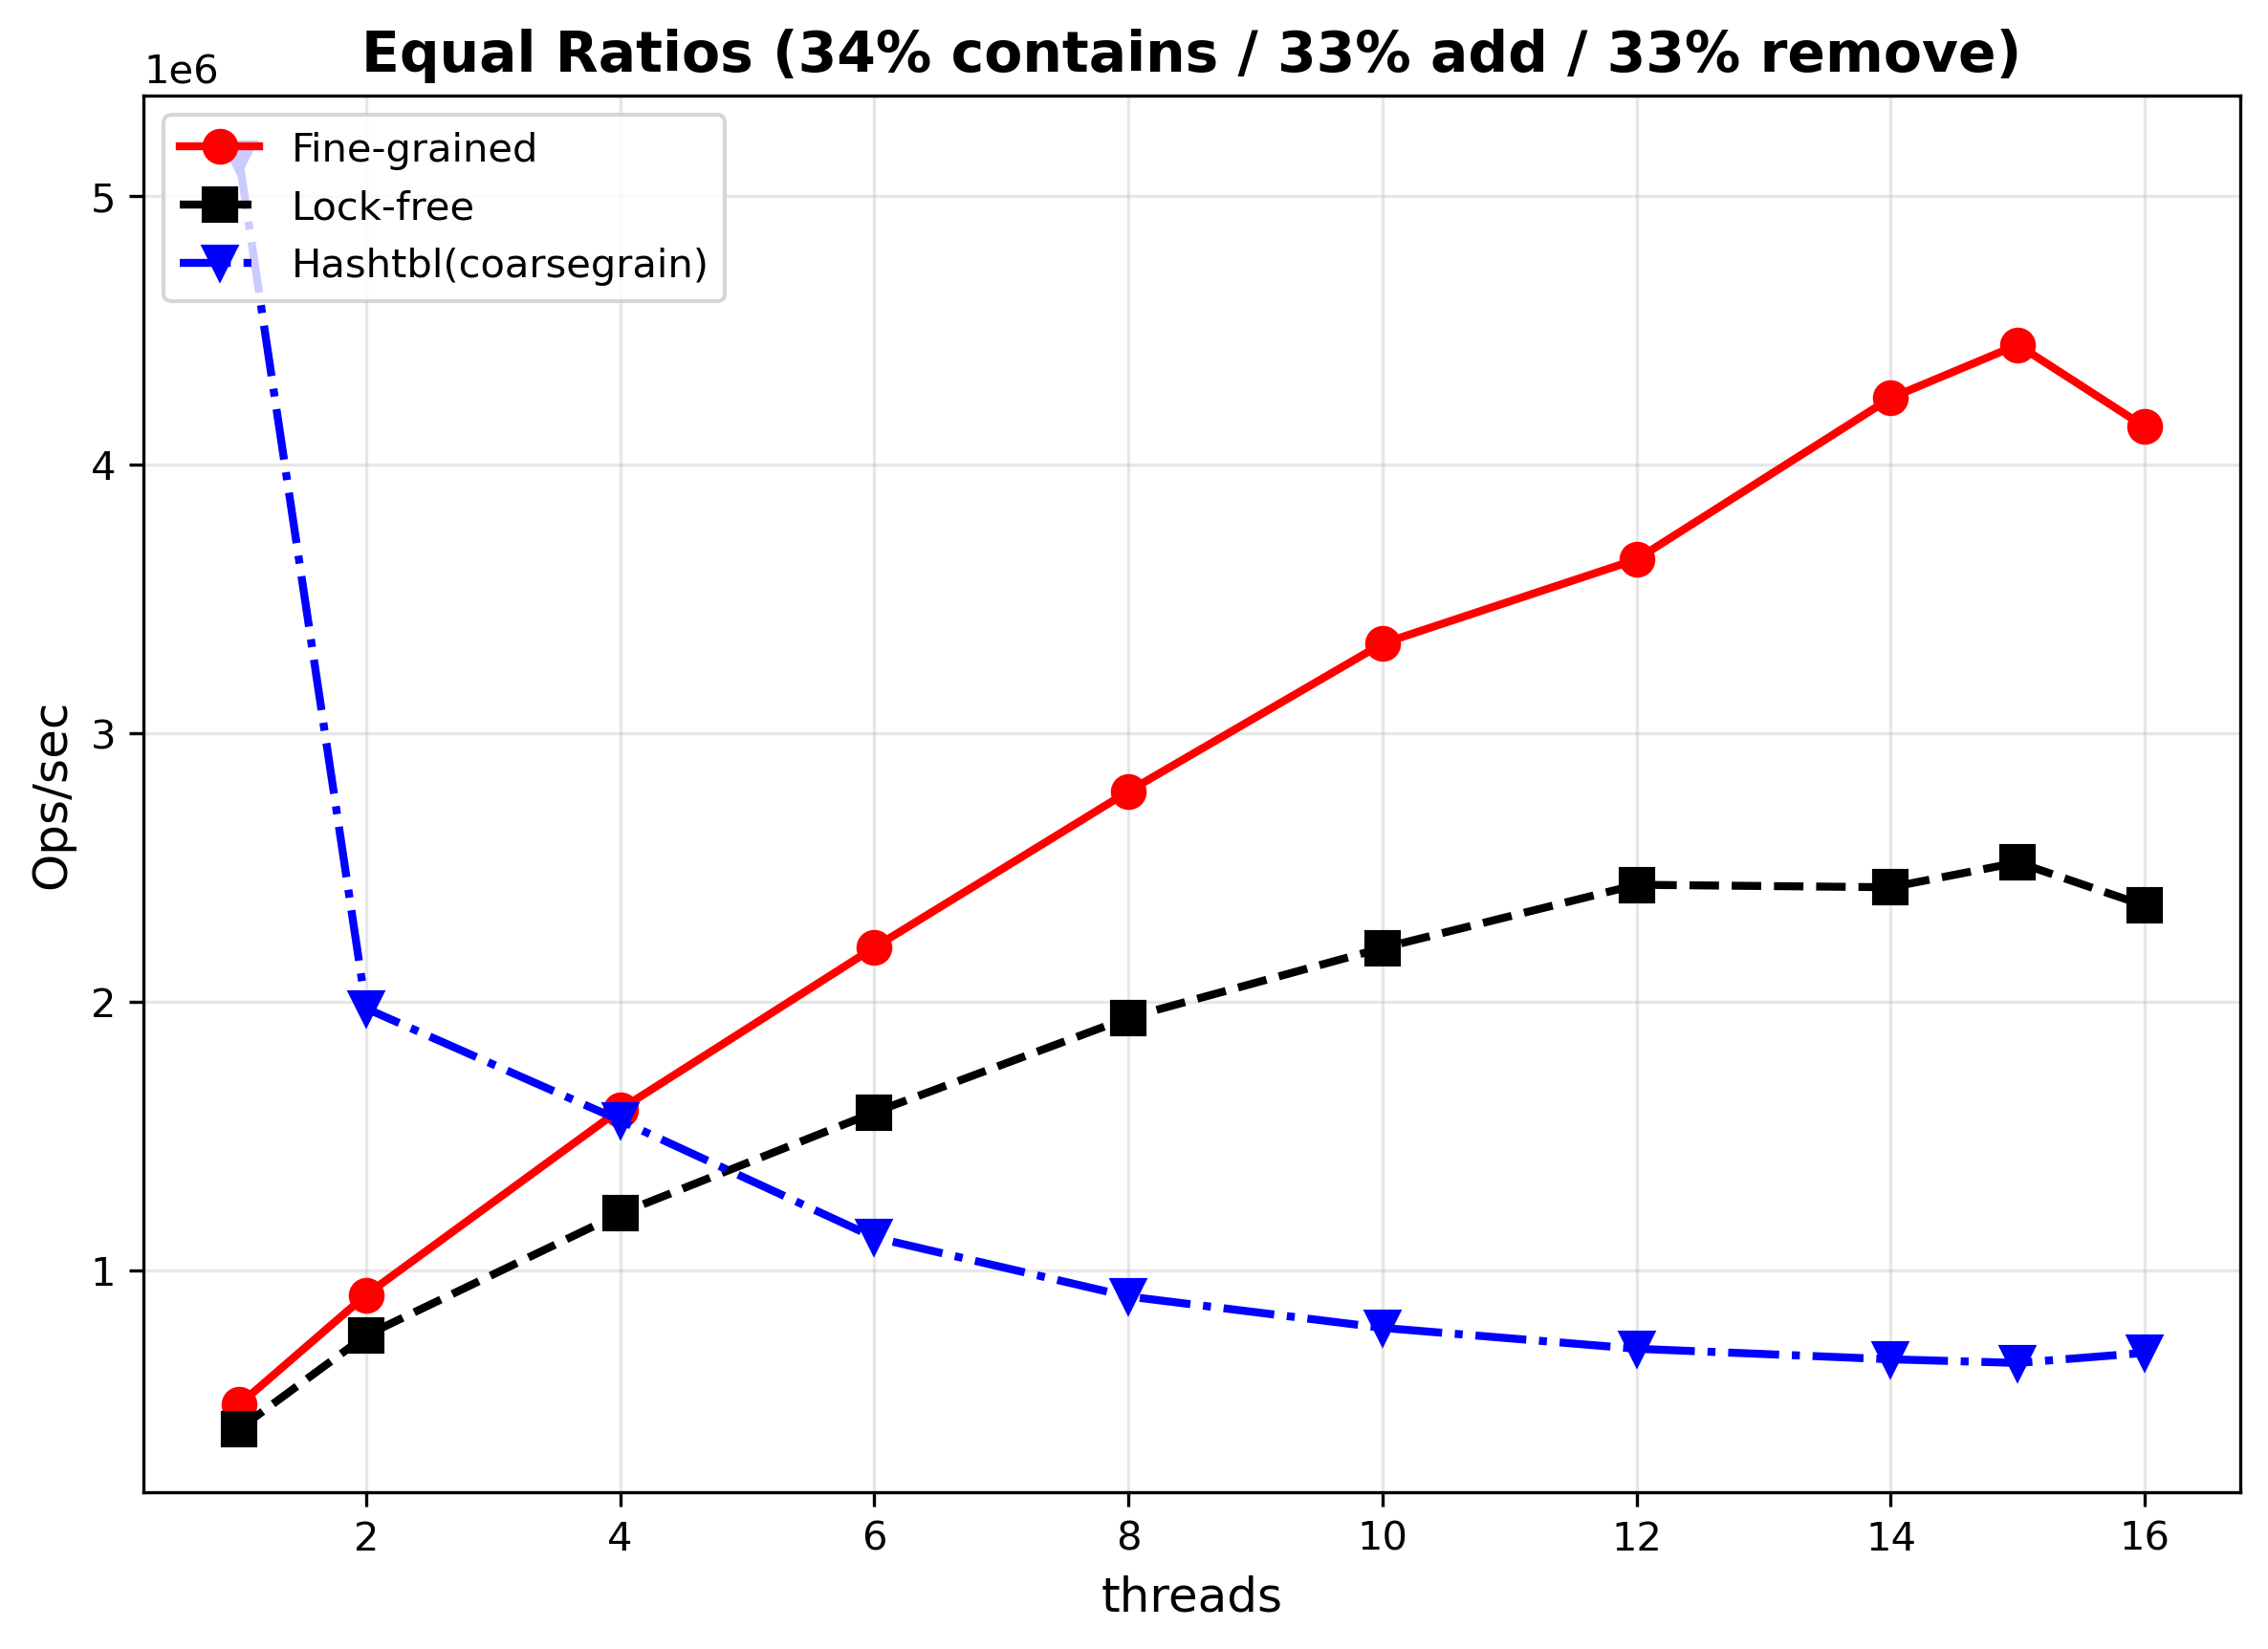
\includegraphics[width=0.85\linewidth]{./plots/plot_equal_ratios.png}
  \caption{Throughput comparison across implementations and thread counts under Equal workload.}
\end{figure}

\begin{figure}[H]
  \centering
  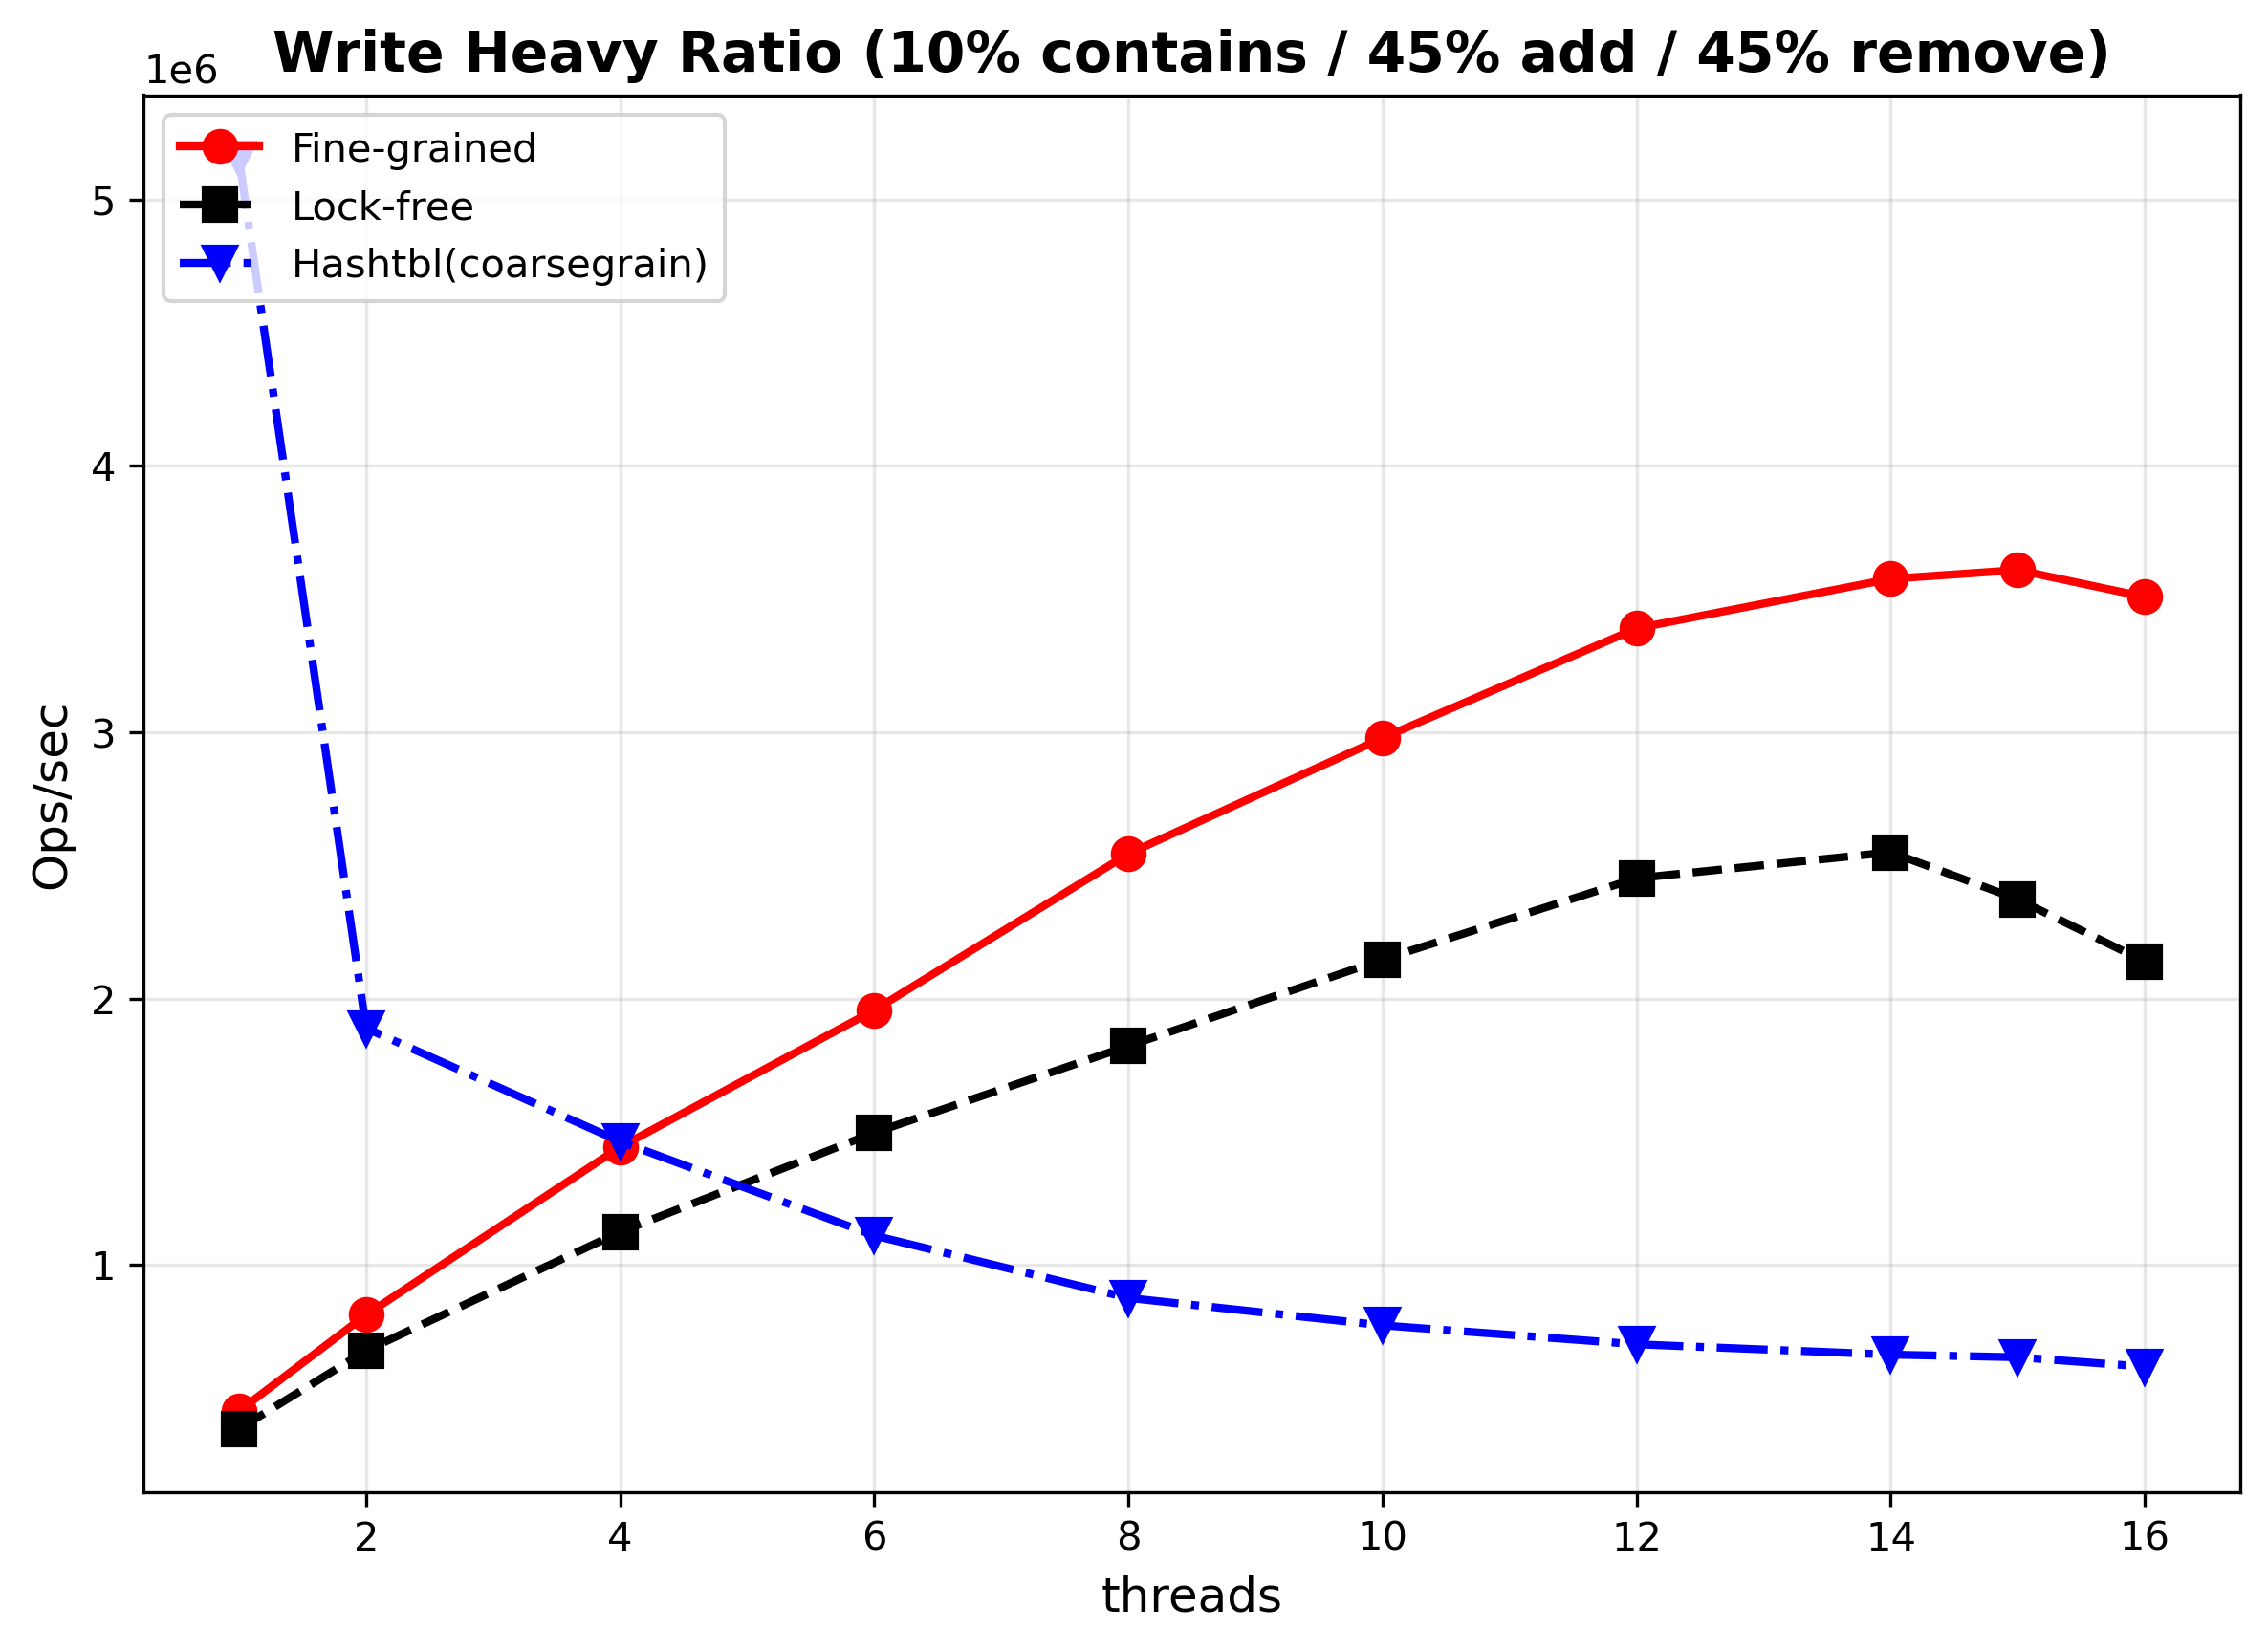
\includegraphics[width=0.85\linewidth]{./plots/plot_write_heavy.png}
  \caption{Throughput comparison across implementations and thread counts under Write-heavy workload.}
\end{figure}

\begin{figure}[H]
  \centering
  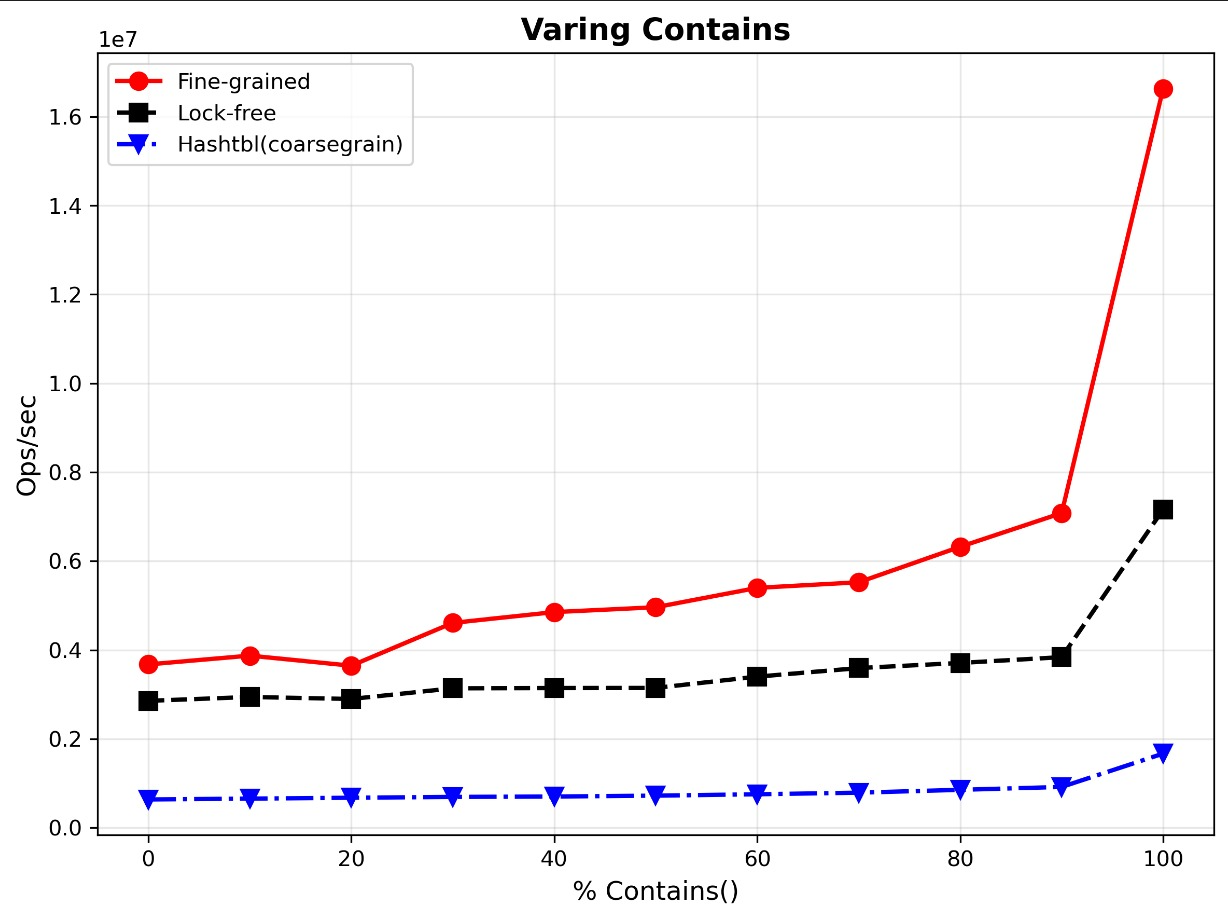
\includegraphics[width=0.85\linewidth]{./plots/image.png}
  \caption{Throughput comparison across implementations and contains load with 10 threads.}
\end{figure}

\subsection{Traversal Length Under Contention}

Like above, we tested three workload mixes to exercise different contention regimes:
\begin{itemize}
  \item \textbf{Read-heavy:} 90\% contains, 5\% add, 5\% remove.
  \item \textbf{Balanced:} 34\% contains, 33\% add, 33\% remove.
  \item \textbf{Write-heavy:} 10\% contains, 45\% add, 45\% remove.
\end{itemize}

\textbf{Measurement methodology}: This benchmark measures the average number of next-pointer traversals (the
``traversal length'') performed by each operation type. For each implementation
we preload the skip list with the configured \texttt{initial\_size}, run a
short warm-up phase and then execute the measured
trial. Unlike the timed throughput benchmark, the traversal benchmark uses a
fixed-count workload: each worker thread performs a fixed number of
operations (the \texttt{runs} parameter) drawn according to the workload mix.
Each operation returns both its result and the number of nodes visited; per-
operation-type sums and counts are accumulated into atomic counters. After all
threads finish we compute the average traversal length per operation as
total-sum / total-count for contains, add and remove. The warm up phase here involves running the same benchmark but for fewer \texttt{runs} parameter (i.e here 1000). In our measurements we assigned \texttt{runs} = 100000.

\begin{figure}[H]
  \centering
  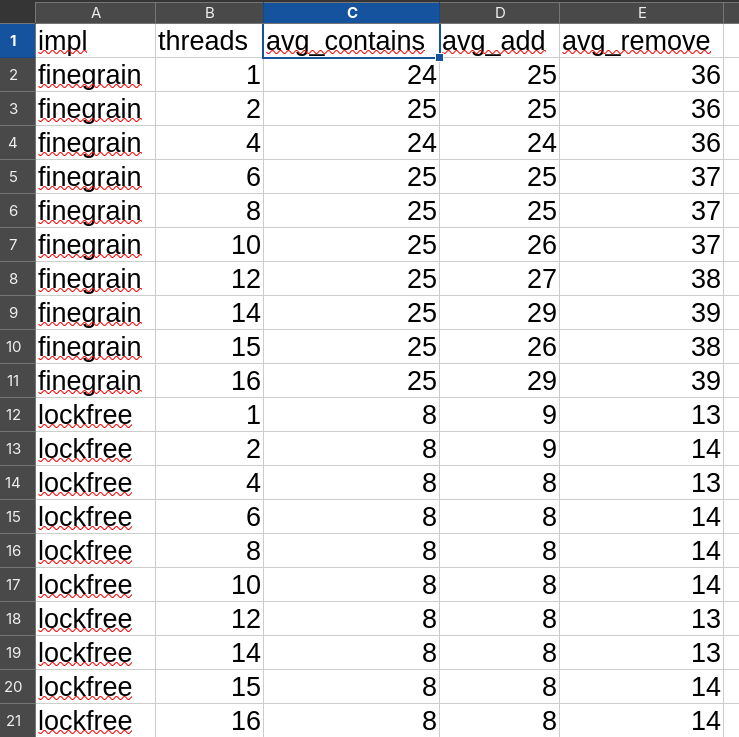
\includegraphics[width=0.85\linewidth,height=0.5\textheight,keepaspectratio]{./plots/tl_reading.png}
  \caption{Average traversal length for Contains, add and remove operations under Read-heavy load.}
\end{figure}

\begin{figure}[H]
  \centering
  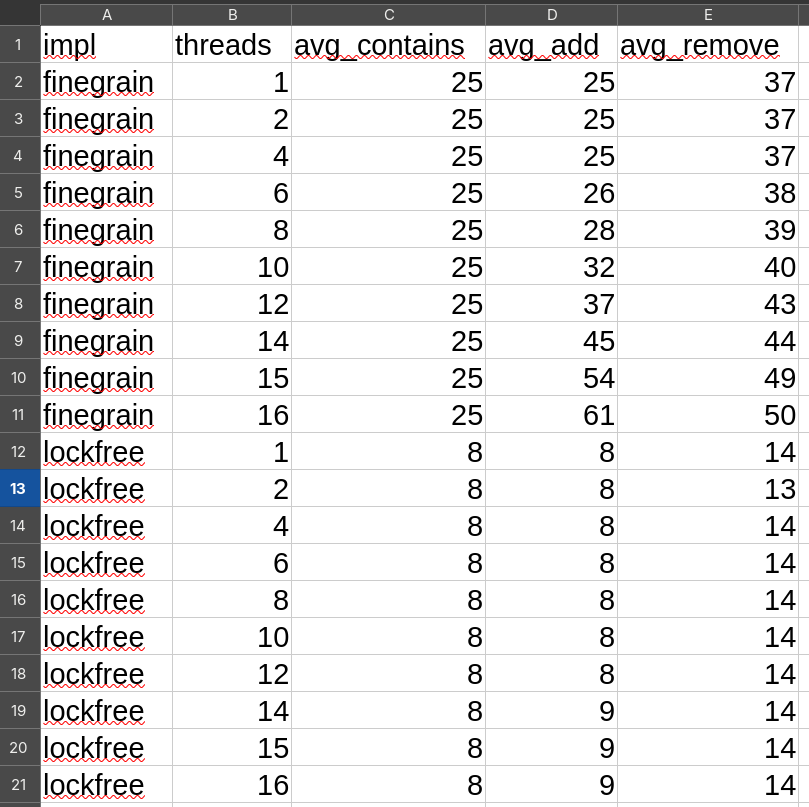
\includegraphics[width=0.85\linewidth,height=0.42\textheight,keepaspectratio]{./plots/tl_equal.png}
  \caption{Average traversal length for Contains, add and remove operations under Equal load.}
\end{figure}

\begin{figure}[H]
  \centering
  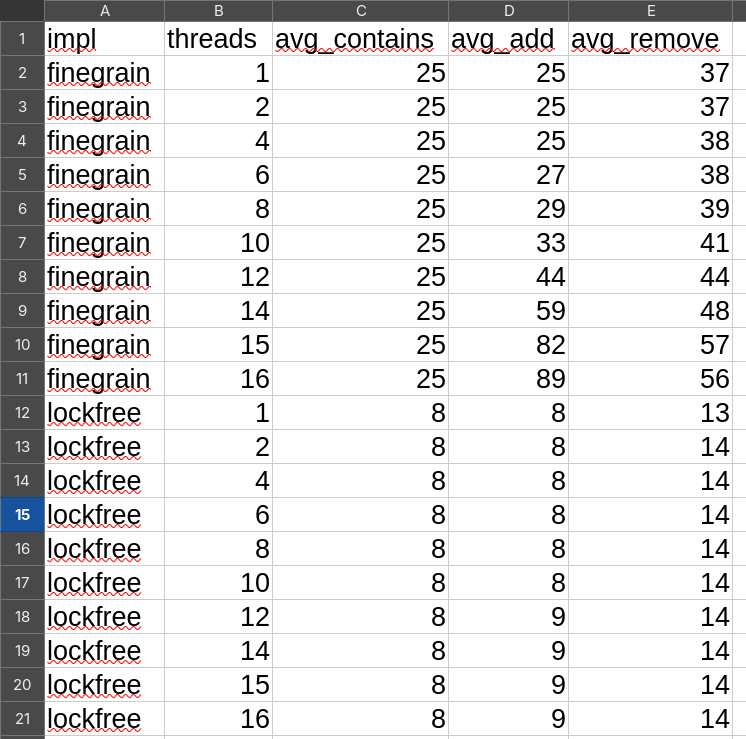
\includegraphics[width=0.85\linewidth,height=0.42\textheight,keepaspectratio]{./plots/tl_writing.png}
  \caption{Average traversal length for Contains, add and remove operations under Write-heavy load.}
\end{figure}

\textbf{Conclusions:} Figure 6-8 show the results of this experiment. To our surprise, the lockfree variant has constant traversal length for each operation across threads. We first thought there might be a bug in our measurement but even after multiple attempts we weren't able find anything different, we came to a conclusion that this might be due to not enough contention being produced beacuse of just 16 threads, as we didn't have access to a machine with higher cores we couldn't test our theory and stick to this conclusion without evidence. Now coming to the finegrain variant, it stays fairly constant till 8-10 threads under equal/write heavy loads then starts to shoot up, implying validation failures during contention and this also explains finegrain variant doesnt grow as rapidly in write heavy loads as compared to read heavy loads in previous experiment. 
% =============================================================================
\section{Reflection on the Use of LLMs}
\label{sec:llm}
% =============================================================================

\paragraph{Tools and models used.}
LLM-backed tools were used throughout the project, mainly ChatGPT, Claude Sonnet 4.6 and Github Copilot in VS-code, with the model set to auto. They were used for understanding the reference algorithms,to go through research papers faster and more efficiently, generating initial code structure, debugging OCaml implementations, designing test cases, interpreting concurrency bugs, and improving the report wording. 

\paragraph{What worked well.}
The LLMs were helpful for explaining the algorithm at a higher level before implementation. In particular, they helped break down the algorithm into traversal, insertion, logical deletion, physical unlinking, and helping. For testing, they helped suggest useful cases such as duplicate insertion, same-key races, high-contention workloads, and comparisons against a sequential model. For the fine-grained and benchmark parts, the LLMs were useful for structuring the code, writing repetitive test cases, and organizing the evaluation section.

\paragraph{What did not work.}
The LLM-generated code could not be trusted directly, especially for subtle synchronization logic. Some suggested checks were redundant, while some explanations around retry logic were too generic. During code review, a few redundant checks in the generated code were identified and removed manually without affecting correctness.The LLMs also sometimes argued for keeping checks that appeared unnecessary; these decisions had to be resolved by reasoning about the algorithm and then validating the implementation.

\paragraph{What was surprising.}
The most surprising part was that the LLMs were often better at explaining the algorithmic idea than at producing reliable concurrent code.They explained the research papers better than the papers. They were useful for understanding temporary states, such as a node being logically deleted but not yet physically unlinked, or a traversal helping another operation complete cleanup. This made it clear that LLM output was useful as guidance, but not as a correctness argument.

\paragraph{What was difficult.}
The difficult parts of the project were the parts where the LLM could not replace understanding: reasoning about interleavings of threads, compare-and-set failures, marked links, and linearisation points. For the lock-free skip list, it was necessary to understand exactly when an operation becomes visible in the abstract set and how helping during traversal changes the structure. For the fine-grained version, care was needed in lock ordering and validation to avoid deadlock and stale snapshots. For the testing and benchmarking parts, the main difficulty was interpreting whether failures or performance differences came from the algorithm, the test design, or the runtime environment.

\paragraph{Overall assessment.}
Overall, the LLMs helped speed up understanding, implementation, debugging, and report writing. However, the results can't be trusted blindly: generated code and explanations were reviewed, simplified where needed, and checked using manual tests, QCheck-STM, QCheck-Lin, ThreadSanitizer, and benchmarks.
% =============================================================================
% \section{Conclusions}
% \label{sec:conclusions}
% % =============================================================================

% Answer the research question stated in \cref{sec:goals}. Summarise the main
% findings. State the limitations of your work honestly. Suggest what you
% would do next given more time.

\section{Conclusions}
\label{sec:conclusions}

The research question asked how the lock-free skip list's throughput scales
relative to a fine-grained locking skip list across different workload mixes,
and whether the multi-level structure amplifies or mitigates the retry overhead
of lock-free operations compared to a single-level Harris list.

The results show that the fine-grained locking skip list consistently
outperforms the lock-free variant across all three workload mixes: read-heavy,
balanced, and write-heavy on our 16-core machine. Both implementations scale
roughly linearly with thread count up to the hardware limit, but the fine-grained
variant exhibits sharper growth, particularly under read-heavy workloads where
its lock-free \texttt{contains} path benefits most. Under write-heavy workloads
the two converge in performance, which the traversal-length experiment helps
explain: under high write contention, the fine-grained variant begins to suffer
increased traversal lengths beyond 8--10 threads due to validation failures and
lock retries, whereas the lock-free variant maintains a near-constant traversal
length across all thread counts. Surprisingly, the lock-free skip list's
traversal length did not grow with contention at all, a result we attribute to
insufficient contention at 16 threads rather than algorithmic superiority, and
one that would need verification on a higher-core machine.

Regarding the second part of the research question, the multi-level structure
of the skip list does not appear to amplify retry overhead beyond what a
single-level Harris list would incur. The \texttt{find} procedure restarts from
the top only on CAS failure during cleanup, and in practice those restarts were
rare enough that traversal lengths remained stable. However, the multi-level
structure does add complexity to the insertion and removal paths, especially
the upper-level splicing in \texttt{add} and the per-level marking in
\texttt{remove}, which may explain why the lock-free variant trails the
fine-grained one: each failed upper-level CAS triggers a fresh \texttt{find}
call, whereas the fine-grained variant's locked region makes those upper-level
updates unconditional once the predecessor locks are held.

The coarse-grained hash table baseline confirmed the expected pattern: it leads
at very low thread counts due to its simplicity and cache locality, but
degrades quickly as contention on the single global mutex grows.

\paragraph{Limitations.}
All experiments were limited to 16 cores; the observed plateau at high thread
counts, and the unexpectedly flat traversal lengths of the lock-free variant,
may look different on a machine with 32 or 64 cores. The value range (10\,000)
and initial size (1\,000) were fixed, so results may not generalise to very
large or very sparse sets.

\paragraph{Future work.}
Given more time we would test on higher-core hardware to confirm whether
lock-free traversal lengths truly stay flat or eventually grow with contention.
We would also experiment with different randomization functions to improve performance while accounting for their computational overhead. Finally, extending both implementations to support
range queries would be a natural next step, since the sorted structure of a
skip list makes range queries significantly cheaper than in a hash table.

% =============================================================================
\section*{Contributions}
\label{sec:contributions}
% =============================================================================

% Required. Percentages must sum to 100. Every member should contribute.

\begin{center}
\begin{tabular}{@{}lcl@{}}
\toprule
\textbf{Member} & \textbf{Contribution (\%)} & \textbf{Main responsibilities} \\
\midrule
Disha & 33\% & Lock-free implementation,Manual tests,TSAN verification \\
Nithin   & 33\% & Lock based implementations,QCheck-Lin and QCheck-STM tests \\
Ved & 34\% &  Benchmarking,Baseline hashtbl implementation \\
\midrule
\textbf{Total} & \textbf{100\%} & \\
\bottomrule
\end{tabular}
\end{center}

% =============================================================================


\bibliographystyle{plainurl}
\bibliography{references}
% =============================================================================

\end{document}
